%\documentclass[twocolumn,twoside]{article}
\documentclass[twoside,twocolumn, letterpaper]{article}
\usepackage{graphics}
\usepackage{color}
\usepackage{NatGenArtT}
%\usepackage{NatureLetT}
\usepackage{times}
\DeclareMathAlphabet{\msfsl}{OT1}{cmss}{m}{sl}
\DeclareMathAlphabet{\msfrg}{OT1}{cmss}{n}{sl}
\renewcommand{\baselinestretch}{1}
\addtolength{\oddsidemargin}{-.2cm}
\addtolength{\evensidemargin}{-1.2cm}
\addtolength{\textwidth}{1.5cm}
\addtolength{\topmargin}{-1.75cm}
\addtolength{\textheight}{3.5cm}
\renewcommand{\textfraction}{0.01}
\renewcommand{\topfraction}{0.99}
\renewcommand{\bottomfraction}{0.65}
\renewcommand{\floatpagefraction}{0.90}
\renewcommand{\dbltopfraction}{0.95}
\renewcommand{\dblfloatpagefraction}{0.80}
\renewcommand{\sfdefault}{phv}

%added commands YANG
\newcommand{\sme}[1]{\textcolor{red}{\bf #1}}
\newcommand{\yang}[1]{\textcolor{cyan}{\emph{\bf  #1}}}
\newcommand{\jri}[1]{\textcolor{red}{\emph{ #1}}}
\graphicspath{{Figure_Table/}} % Location of the graphics files

\makeatletter
\renewcommand{\footnotesep}{-2pt}
\makeatletter

\usepackage{fancyhdr}
\pagestyle{fancy}
\fancyhf{}

% fancy for Nature Genetics
\fancyhead[RO]{\begin{picture}(600,1)(10,20)\put(440,32) {\textcolor{Dgreen}{\large{\sfbf{ARTICLES}}}}\end{picture}}
\fancyhead[RE]{\begin{picture}(600,1)(10,20)\put(10,32)  {\textcolor{Dgreen}{\large{\sfbf{ARTICLES}}}}\end{picture}}
\fancyhead[C]{\begin{picture}(600,1)(10,20)\linethickness{50pt}\put(-43,52) {{\color{pTop}{\line(1,0){615}}}}\linethickness{0.5pt}\put(10,-678) {{\line(1,0){515}}}\end{picture}}

% fancy for Nature
%\fancyhead[RO]{\begin{picture}(600,1)(10,20)\put(460,46) {\textcolor{Dgreen}{\stbld{LETTERS}}} \put(10,46) {\textcolor{Dgreen}{\sf{NATURE}}} \end{picture}}
%\fancyhead[RE]{\begin{picture}(600,1)(10,20)\put(10,46) {\textcolor{Dgreen}{\stbld{LETTERS}}} \put(460,46) {\textcolor{Dgreen}{\sf{NATURE}}} \end{picture}}
%\fancyhead[C]{\begin{picture}(600,1)(10,20)\linethickness{25pt}\put(-43,54) {{\color{pTop}{\line(1,0){615}}}}\linethickness{0.5pt}\put(10,-678) {{\line(1,0){515}}}\end{picture}}

\fancyfoot[RO]{\thepage}
\fancyfoot[LE]{\thepage}

\renewcommand{\headrulewidth}{0pt}
\fancypagestyle{plain}{
    \fancyhf{}
}
\setcounter{footnote}{0}%

\title{Incorporation of Evolutionary Constraint Improves Genomic Prediction of Hybrid Phenotypes}


\author{
Jinliang Yang\thanks{Department of Plant Sciences, University of California, Davis, CA 95616, USA} $^,$\thanks{These authors contributed equally to this work} \hspace{0.5mm}, 
Sofiane Mezmouk$^{1,2,}$\thanks{Current address: KWS SAAT AG, Grimsehlstr. 31, 37555 Einbeck, Germany} \hspace{0.5mm}, 
Andy Baumgarten\thanks{DuPont Pioneer, Johnston, IA 50131, USA} \hspace{0.5mm}, 
Edward S. Buckler\thanks{US Department of Agriculture, Agricultural Research Service, Ithaca, NY 14853, USA} \hspace{0.5mm}, 
Katherine E. Guill\thanks{US Department of Agriculture, Agricultural Research Service, Columbia, MO 65211, USA} \hspace{0.5mm},
Michael D. McMullen$^{6,}$\thanks{Division of Plant Sciences, University of Missouri, Columbia, MO 65211, USA} \hspace{0.5mm},
Rita H. Mumm\thanks{Department of Crop Sciences, University of Illinois at Urbana-Champaign, Urbana, IL 61801, USA} \hspace{0.5mm},
and Jeffrey Ross-Ibarra$^{1,}$\thanks{Center for Population Biology and Genome Center, University of California, Davis, CA 95616, USA} $^,$\thanks{Correspondence should be addressed to J.R-I. (rossibarra@ucdavis.edu).}\hspace{0.5mm}
}
\date{\small Manuscript intended for \emph{Nature Genetics}, \today}



\usepackage[sort&compress]{natbib}
\bibpunct{}{}{,}{s}{}{\textsuperscript{,}}

\usepackage{amsmath}
\usepackage{graphicx}

\begin{document} 
\maketitle

\begin{abstract}
\noindent \bf
\noindent
Complementation of deleterious alleles has long been proposed as a major contributor to the hybrid vigor observed in offspring of inbred parents. 
We test this hypothesis using evolutionary measures of sequence conservation to ask whether incorporating information about putatively deleterious alleles can inform genomic selection (GS) models and improve phenotypic prediction.
We measured a number of agronomic traits in both the inbred parents and hybrids of an elite maize partial diallel population. 
We resequenced the parents of the population, using genomic evolutionary rate profiling (GERP) to identify constrained sites across more than 86 Mb sites across the genome.  
We identifed haplotype blocks using an identity-by-decent (IBD) analysis and scored these blocks on the basis of segregating putatively deleterious variants. 
As a result, incorporating sequence conservation improves prediction accuracies in a five-fold cross-validation experiment for several traits \emph{per se} as well as heterosis for those traits. 
These results provide strong empirical support for the simple complementation model of heterosis, and demonstrates the utility of incorporatin functional annotation and its potential usage in phenotypic prediction and plant breeding. 

\end{abstract}

\vspace{6mm}




%%%%%%%%%%%%%%%%%%%%%%%%%%%%%%%%%%%%%%%%%%%%%%%%%%%%%%%%%%%
\noindent %\textbf{Why we care about deleterious variants. Discuss results of Mezmouk 2014. We are extending this in three ways}  
%\begin{itemize}
%  \item all deleterious SNPs not just coding
%  \item genome-wide not just reduced representation
%  \item using GS to test whether they improve prediction
%\end{itemize}

The phenomenon of heterosis or hybrid vigor has been observed across many species, from yeast \cite[]{Shapira2014} to plants \cite[]{shull1908composition} and vertebrates \cite[]{Gama2013}. 
Hybrid vigor is particularly important in agriculture, where hybrid breeding is fundamental to the production of a number of crops including both rice \citex and maize \citex .
A number of hypotheses have been put forth to explain the phenomenon, including gene dosage \cite[]{birchler2003search}, overdominance \cite[]{east1936heterosis, schwartz1973single, krieger2010flowering}, 
%pseudo-overdomiance \cite[]{graham1997characterization, McMullen2009}, 
and epistasis \cite[]{minvielle1987dominance, schnell1992multiplicative}. 
Complementation of recessive deleterious alleles, however, remains the simplest genetic explanation \cite[]{Charlesworth2009}, and one that is supported by considerable empirical evidence \citex \cite[]{xiao1995dominance, frascaroli2007classical}.
\jri{i'm not sure these are all appropriate. huang2015genomic for example i think doesn't actually measure heterosis, they just do GWAS on hybrids. and frascaroli if I read it right says that heterosis for grain yield is mostly overdominance (dominance $>1$).}

%One of the best studied examples of hybrid vigor is that of maize. 
%Hybrid maize has formed the basis of modern maize agriculture since the early 20th century \cite[]{crow1998}. 

%Cr the benefits of cross-fertilization or hybridization were not unknown, it was not until the early 20th century that East, Shull, and others demonstrated the utility of hybrid breeding for  in the past, it was not until the early 20th century that hybridwork of Shull, East, and others that it's significance for agriculture was well appreciated \citex.
%Now, hybrid seed makes up the vast majority \jri{in progress, still reading}


%Deleterious alleles were arisen from new mutations during meiosis. In maize, about 90 new mutations were generated per meiosis \cite[]{Clark2005}, majority of which were deleterious according to empirical estimates \cite[]{Joseph2004}. In a natural outcross population, the negative effects on fitness of these deleterious alleles make them subject to be selection against, which lead the deleterious alleles to be maintained in a low frequency \cite[]{Eyre-Walker2007}. But the deleterious alleles could not be completely purged. 

%In maize, the total number of mildly deleterious mutations is substantial because of the exponential growth of population size after domestication. The modern breeding probably aims to remove these deleterious mutations and pyramiding beneficial alleles for agronomical purposes. In practice, the relatively homogeneous maize germplasm pool was artificially divided into different heterotic groups \cite[]{Heerwaarden2012}. It enabled the improvement of germplasm pools to be conducted in a parallel fashion, and therefore, facilitated the breeding efficiency. Using this hybrid breeding approach, the maize yield has been steadily improved since the early 20th century \cite[]{duvick2001biotechnology}. However, removing deleterious mutations in low recombination regions or in tightly linked regions become less effective. Studies indicated that residual heterozygosity correlates negatively with recombination \cite[]{Gore2009, McMullen2009} and the low recombination is effective over long period of time \cite[]{Haddrill2007}. As a consequence, the deleterious alleles would be accumulated in the low recombination regions, such as the pericentromeric regions in maize, and the vigorous performance could be realized by combining two sets of non-deleterious or beneficial alleles in repulsion state, thus lead to pesudo-overdominance. A recent QTL study identified loci controlling for heterosis are enriched in centromeric regions \cite[]{Lariepe2012}, which partly support this pesudo-overdominance hypothesis.

%Despite the importance of deleterious alleles in contributing to heterosis, they have not been systematically investigated probably because of their low frequencies in the population and mostly exhibiting minor effects. Here, we employed a genomic selection (GS) approach to simultaneously estimate genome-wide deleterious variants in a half diallel population. The diallel population was composed of a set of hybrids, which enabled us to explore different modes of inheritance of the deleterious variants. And the study can be conducted with millions of variants but using relative little sequencing efforts. In our previous study, deleterious SNPs were found to be enriched in a SNP set identified by GWAS \cite[]{Mezmouk2014}. The deleterious variants in the study were defined as non-synonymous mutations in the coding regions. Clearly, deleterious variants are not limited to coding regions. Here, we expanded the characterization of deleterious variants to genome-wide using genomic evolutionary rate profiling (GERP) \cite[]{Cooper2005}. By incorporating GERP information in GS models, we demonstrated the prediction accuracies were significantly improved not only for some traits \emph{per se}, but aslo for some heterosis transformations (especially for traits exhibiting high levels of hereosis). Further studies indicated that joint effects of deleterious alleles with additive and dominant modes of inheritance may contribute to heterosis.



%%%%%%%%%%%%%%%%%%%%%%%%%%%%%%%%%%%%%%%%%% FIGURE
\begin{figure*}[tb]   
  \begin{center}
   \vspace{-2mm}
   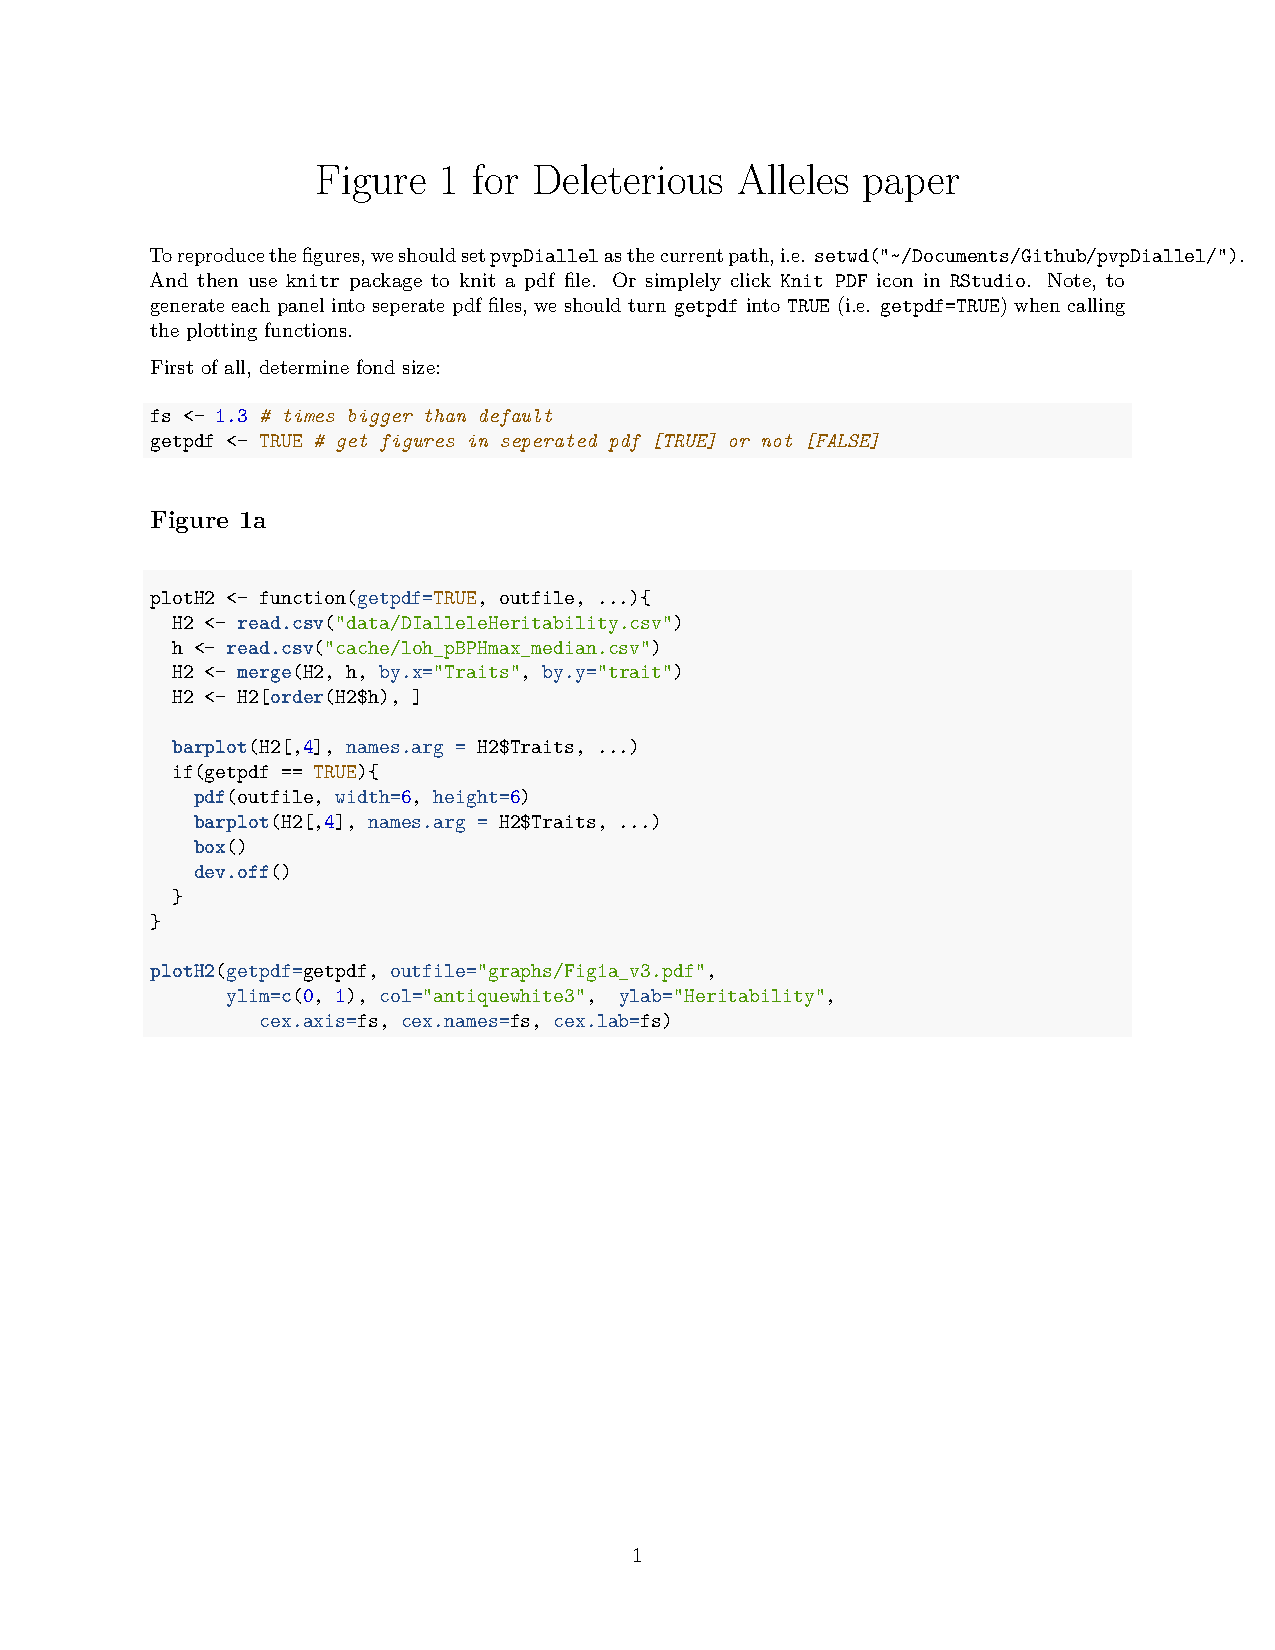
\includegraphics[width=0.8\textwidth]{fig/Fig1}
   \renewcommand{\baselinestretch}{0.9}
   \vspace{-3mm}
   \caption{({\bfseries a-b}) Demonstrating the performance of Feil et al.'s method \cite[]{Feil_1999_10555280,Feil_2000_10747043} for estimating the relative rate of homologous recombination ($g/\mu$). The effect of population (clonal) structure is investigated using the model illustrated in ({\bfseries a}), which considers 50 subpopulations that share an ancestral population. Migration among the subpopulations is allowed, and the migration rate represents the level of population structure. It is shown that $g/\mu$ is highly underestimated when the migration rate is small, while $g/\mu$ is well estimated when the entire population is less structured ({\bfseries b}). 
({\bfseries c}) Distribution of the estimates of the relative recombination rate ($g/\mu$) in 48 bacterial species, summarized by Vos \& Didelot \cite{Vos_2009_18830278}. Note that we use this data set \cite{Vos_2009_18830278} based on Didelot \& Falush's method \cite[]{Didelot_2007_17151252} because estimates by Feil et al.'s method are available for far fewer species \cite[]{Narra_2006_16950097}. We verified the correlation of the estimates obtained by the two methods, as we show later.} 
\vspace{-4mm}
    \label{Feilmethod}
  \end{center}
\end{figure*}
%%%%%%%%%%%%%%%%%%%%%%%%%%%%%%%%%%%%%%%%%% FIGURE

While this can be possible for model species with genome-wide SNP data such as Drosophila and Arabidopsis \cite[]{Haddrill_2005_15930491,Plagnol_2006_16299388}, it is difficult for bacteria that usually have strong and complex clonal population structure. Therefore, several \emph{ad hoc} methods have been developed \cite{Feil_1999_10555280,Feil_2000_10747043}, which are designed to minimize the effect of demography. In practice, these methods focus on very recent variations and distinguish their causal mechanisms (\emph{i.e.,} mutation vs. homologous recombination), from which the relative rate of homologous recombination and mutation is estimated. Because such recent events are indeed robust to demographic effects, application of these methods has provided improved estimates using large-scale sequence variation data, such as those made available by the multilocus sequence typing (MLST) project, in which short fragments in seven housekeeping genes were resequenced for a large sample from various species \cite[]{Maiden_1998_9501229}.

However, a serious problem still remains when clonal structure is very strong, as illustrated in {\bf Fig.~\ref{Feilmethod}}. To demonstrate the point, we assumed a very simple model with multiple clonal subpopulations, among which migration is allowed ({\bf Fig.~\ref{Feilmethod}a}). When the migration rate is low, it is considered that the population has strong clonal structure, while individuals in the entire population behave as if it is panmictic with frequent migration. We assumed that the rates of homologous recombination ($g$) and mutation ($\mu$) are identical, so that the true relative rate ($g/\mu$) is 1. Then, genotype data that are similar to the MLST data were generated by coalescent simulations using the {\sf ms} software \cite[]{Hudson_2002_11847089}, and the relative rate of homologous recombination was estimated by using Feil et al.'s method \cite{Feil_1999_10555280,Feil_2000_10747043}. We found that the rate was well estimated under 
the assumption of frequent migration, yet was highly underestimated under a strong clonal structure. Further, it seems that the method has very limited power to detect recombination when the population is highly structured ({\bf Fig.~\ref{Feilmethod}b}). This is because recombination can be detected only when the exchanged sequences have accumulated sufficient nucleotide variation. In each clonal population, where the genomic sequences of all individuals are very similar, most recombination events are not detectable. This reasoning also holds for the method of Didelot and Falush \cite[]{Didelot_2007_17151252}, which preferentially detects recombined regions from highly diverged clones. Therefore, we hypothesize that the estimated rates of homologous recombination thus far could be much lower than the
 true rates in natural populations, particularly for species with strong clonal structure. 

 In this study, we set out to verify this hypothesis by re-evaluating the homologous recombination rate in bacteria, mainly focusing on 
 a species with strong clonal structure, given that, for such species, the extent of underestimation in the homologous recombination rate would be 
 significant  ({\bf Fig.~\ref{Feilmethod}}). Based on this rationale, we chose \emph{Staphylococcus aureus} as a model organism. \emph{S. aureus} is a major pathogen that is associated with serious community-acquired and nosocomial diseases \cite[]{Emori_1993_8269394,Steinberg_1996_49}. Methicillin-resistant strains (MRSA) of this species are well recognized because they are resistant to multiple antibiotics, including methicillin, and their infection could cause serious diseases \cite[]{Panlilio_1992_51,Speller_1997_52,Grubb_1998_50}. Due to these medical concerns, \emph{S. aureus} is one of the species for which genomic sequences of multiple individuals are available; whole-genome sequences for this species are available for more than ten strains, including MRSA and MSSA (methicillin-susceptible \emph{S. aureus}) strains ({\bf Supplementary Table~1}). It has long been believed that \emph{S. aureus} has very strong clonal structure \cite[]{Musser_1990_1967495,Musser_1992_53,Feil_2003_12754228,Cooper_2006_16622047}. Previous analyses indicated that recombination rate in \emph{S. aureus} is very low. The ratio of the homologous recombination rate to the mutation rate ($g/\mu$) in this species was estimated to be about 0.067 \cite[]{Feil_2003_12754228} by Feil et al.'s method \cite{Feil_1999_10555280,Feil_2000_10747043}. Narra and Ochman \cite[]{Narra_2006_16950097} classified 23 bacterial species into three categories (high, medium, and low) according to the recombination rate estimated by Feil et al.'s method, and placed \emph{S. aureus} 
 in the `low' category.
Vos \& Didelot \cite{Vos_2009_18830278} summarized estimates of the relative homologous recombination rate ($g/\mu$) for 48 bacterial species using the method of Didelot and Falush \cite[]{Didelot_2007_17151252}. The estimate for \emph{S. aureus} was $g/\mu$ = 0.1, which was the second lowest among the 48 species (see {\bf Fig.~\ref{Feilmethod}c} for the distribution of estimates for the 48 species). Thus, \emph{S. aureus} provides an appropriate model organism for our purpose of evaluating the homologous recombination rate in a highly structured population. 
 If our hypothesis turned out to be correct, the low estimates for this species would not be true, but rather a mere result of underestimation due 
  to the strong population structure. 

%%%%%%%%%%%%%%%%%%%%%%%%%%%%%%%%%%%%%%%%%% FIGURE
\begin{figure*}[tb]   
  \begin{center}
   \vspace{-2mm}
   \includegraphics[width=0.8\textwidth]{fig/treeCircle}
   \renewcommand{\baselinestretch}{0.9}
   \vspace{-3mm}
   \caption{\sfbf{Genome-wide pattern of homologous recombination in \emph{S. aureus}.}
   (\textbf{a}) An NJ tree of the 12 strains in \emph{S. aureus} based on the distance matrix of all synonymous SNPs. The 12 strains were classified into 5 groups, named A, B, C, D and E. (\textbf{b}) The proportions of different tree-shapes.  (\textbf{c}) The distribution of tree-shapes across the genome. (\textbf{d}) Local patterns of gene trees in three representative regions with length 10 kb. Gray boxes represent coding genes. For each gene, an NJ tree was constructed if no evidence for recombination was detected by the four-gamete test \cite[]{Hudson_1985_4029609}, otherwise the gene region was divided into blocks at putative recombination breakpoints and a tree is shown for each block.
   }
\vspace{-4mm}
    \label{circle}
  \end{center}
\end{figure*}
%%%%%%%%%%%%%%%%%%%%%%%%%%%%%%%%%%%%%%%%%% FIGURE

 In this study, we used a population genetics approach that would provide a more accurate estimate (robust to demography) as long as reasonable demography was assumed. We first inferred the demographic history and then estimated the rate of homologous recombination 
 conditional on the inferred demography. While this approach has been applied quite successfully to model eukaryotic species with abundant SNP data \cite[]{Haddrill_2005_15930491,Plagnol_2006_16299388}, its application to bacteria with complex population 
 structures is not straightforward. Therefore, when applied to \emph{S. aureus}, rather than using all strains, we focused only on a subset,
 which allowed us to use the coalescent framework for analyses and simulations. 
% within which the coalescent process is simple enough to 
%  between which the coalescent process should be simple enough to treat in the framework of the coalescent theory with less complicated %settings. 
 To this end, we show that the relative rate of recombination is about 10 times larger than the previous estimates. Our results imply  
 that bacteria could undergo much higher rates of homologous recombination than previously thought, postulating an important role 
 for this process in bacterial genome evolution. To validate this postulation, we investigated the  evolutionary significance of 
 homologous recombination. 
 It is widely accepted that recombination is evolutionarily advantageous because it can break down linkage between loci and subsequently create new combinations of alleles \cite[]{Felsenstein_1974_4448362, MaynardSmith78:book, Kondrashov_1993_8409359, Barton_1998_9748151, Otto_2002_11967550}, an argument that is frequently used to explain the existence of two sexes. As such, the common assumption that the evolution of asexual species, such as bacteria, is largely clonal and does not utilize recombination, puts such species at an evolutionary disadvantage in at least two scenarios. In the first scenario, known as ``clonal interference" of beneficial mutations, when two beneficial mutations arise simultaneously in different individuals, it is impossible that both of them fix in the population because when one fixes, the other has to be lost \cite[]{Fisher30:book, Muller_1932_62, Hill_1966_37, Gerrish_1998_9720276}. In the second scenario, deleterious mutations likely fix in the population. For example, through the ``hitchhiking" effect, when a beneficial mutation fixes by positive selection, linked deleterious mutations also fix \cite[]{Kojima_1967_4, Maynard_Smith_1974_5}. The effect of background selection can be maximized with no recombination because of a high proportion of individuals having strongly deleterious mutations, causing a serious reduction in the effective population size. As a consequence, deleterious mutations have a high chance to fix by genetic drift \cite[]{Charlesworth_1993_8375663}. An extreme case of this would be the situation known as Muller's ratchet; if the deleterious mutation rate is so high that all individuals have at least one deleterious mutation, then at least one of them will eventually fix in the population \cite[]{Muller_1932_62, Muller_1964_31}. 

It may be possible that bacteria can overcome, by utilizing homologous recombination, the aforementioned evolutionary disadvantage scenarios, but this possibility has not been systematically investigated due to the lack of knowledge on the rate of recombination in natural populations. Instead, a view to the contrary has been provided:
 %negative view was provided when the role of homologous recombination was underappreciated: 
 since homologous recombination affects very limited genomic regions, it may not have sufficient power to relax those evolutionary disadvantages \cite[]{MaynardSmith_1991_1985260}. The role of homologous recombination  has gained more appreciation, 
 but its evolutionary advantages are still under debate, and the arguments are mainly based on experimental evolution studies \cite[]{Souza_1997_64,Cooper_2007_17713986,Bacher_2006_17028281,Baltrus_2008_17976191}. 
To address this issue, here we use simulations as an alternative approach. By simulating bacterial genome evolution with advantageous and deleterious mutations and homologous recombination, we investigated the fixation rates of both types of mutations. Based on the 
simulation results,  we discuss the bacterial population's ability to avoid evolutionary disadvantages by means of homologous recombination.



% Bacterial recombination is usually modeled as allelic gene conversion in eukaryotes \cite[]{Wiuf_2000_10790416,Didelot_2007_17151252}. 


% \emph{S. aureus} is known to have fairly conserved colinearity of the genome within species \cite[]{Lindsay_2004_15276614}, which facilitates the construction of whole-genome alignment. 

% The 55 \% of pairwise comparisons between genes trees of MLST loci show significantly congruent \cite[]{Feil_2003_12754228}.

%The assumption of clonal inheritance, {\em i.e.}, the whole genome is completely linked, has been central to almost all evolutionary theories of asexual species. These theories have provided the basis for analyses of artificial evolution of bacterial populations in the lab, as well as for deriving estimates of their evolutionary parameters, including the rate and fitness effects of mutations \cite[]{Imhof_2001_11158603,Rozen_CB_2002,Hegreness_2006_16543462,Perfeito_2007_17690297}. 


%%%%%%%%%%%%%%%%%%%%%%%%%%%%%%%%%%%%%%%%%% FIGURE
\begin{figure*}[tb]   
  \begin{center}
   \vspace{-2mm}
   \includegraphics[width=0.8\textwidth]{fig/ms}
   \renewcommand{\baselinestretch}{0.9}
   \vspace{-3mm}
   \caption{({\bfseries a}) The demographic model for the A-B-C trio used in this study. ({\bfseries b}) The distributions of the synonymous nucleotide divergence between groups A-C (green boxes in the upper panel), B-C (blue boxes in the upper panel) and A-B (red triangles in the lower panel). The expected distributions under the inferred demography are shown by gray lines. ({\bfseries c}) The decay of linkage disequilibrium (LD). The horizontal and vertical axes represent the distances (kb) between SNPs and the probability of tree-shape compatibility, respectively. The gray circles represent the observation (the proportion of compatible trees for SNP pairs given distance). Distances were binned, and each circle represents the proportion of compatible trees in the same bin. The red line represents the expected decay of LD with the estimated rate, $\msfsl{\hat{G}}$ = 0.006, $\hat{\msfrg{1}\msfsl{/q}}$ = 10 kb.}
\vspace{-6mm}
    \label{demo}
  \end{center}
\end{figure*}
%%%%%%%%%%%%%%%%%%%%%%%%%%%%%%%%%%%%%%%%%% FIGURE

%%%%%%%%%%%%%%%%%%%%%%%%%%%%%%%%%%%%%%%%%% FIGURE
\begin{figure*}[tb]   
  \begin{center}
   \vspace{-2mm}
   \includegraphics[width=0.7\textwidth]{fig/BacLD}
   \renewcommand{\baselinestretch}{0.9}
   \vspace{-1mm}
 \caption{Decay of LD ($r^2$) in various bacterial species. In addition to \emph{S. aureus} ({\bfseries a}), eight species (\emph{Bacillus cereus}, \emph{Campylobacter jejuni}, \emph{Clostridium botulinum}, \emph{Escherichia coli}, \emph{Helicobacter pylori}, \emph{Salmonella enterica}, \emph{Streptococcus pneumoniae}, and \emph{Streptococcus pyogenes}) were analyzed ({\bfseries b$\sim$i}). In all species, LD decays quite dramatically and saturates in several kb. The saturated level of LD ($\msfsl{LD_{\infty, obs}}$) is roughly shown by a red broken line, which is usually higher than the level expected between completely unlinked SNPs ($\msfsl{LD_{\infty, exp}}$, blue broken line), possibly due to population structure.  ({\bfseries j}) $\msfsl{LD_{\infty, obs}/LD_{\infty, exp}}$ in seven species, for which estimates of the recombination rate ($g/\mu$) are available in Narra and Ochman \cite[]{Narra_2006_16950097}.  ({\bfseries k}) $\msfsl{LD_{\infty, obs}/LD_{\infty, exp}}$ in all nine species, plotted against estimates of $g/\mu$ by Didelot \& Falush's method \cite[]{Didelot_2007_17151252} (data from Vos \& Didelot \cite{Vos_2009_18830278}).}
\vspace{-6mm}
    \label{BacLD}
  \end{center}
\end{figure*}
%%%%%%%%%%%%%%%%%%%%%%%%%%%%%%%%%%%%%%%%%% FIGURE
\section*{RESULTS}
\subsection*{Evaluating the homologous recombination rate in \emph{S. aureus}}
The whole-genomic sequences of 12 strains of \emph{S. aureus} were obtained from the NCBI database (ftp://ftp.ncbi.nih.gov/genomes/). \emph{S. aureus} has a circular genome, and the genome sizes of the 12 strains range from 2.74Mb to 2.91Mb. These strains were isolated from humans, except for RF122, which was isolated from a bovine. The 12 strains consist of 8 methicillin-resistance (MRSA) and 4 methicillin-susceptible (non-MRSA) strains ({\bf Supplementary Table~1}). The genomes were aligned and 65,412 SNPs were identified in 2.3 Mb of well-aligned regions, which cover more than 80 \% of the entire \emph{S. aureus} genome (on average, $\sim$2.8 Mb; {\bf Supplementary Methods} online). The average pairwise nucleotide differences per site is $\pi=0.00847$ for all sites, and $\pi_S=0.0247$ for synonymous sites ({\bf Supplementary Methods} online).

Estimation of the homologous recombination rate from polymorphism data is difficult without knowing the demographic history of the population. This is especially true for bacterial populations that usually have strong clonal structure \cite[]{Selander_1980_56,Orskov_1983,Hartl_1984_47,Smith_1993_8506277}. Indeed, the relationship of the 12 strains is very different from that expected when the sample is from a panmictic population. {\bf Fig.~\ref{circle}a} shows an NJ tree based on the distance matrix of all synonymous SNPs. This tree represents the genome-wide average of tree structure of the 12 strains, and indicates that the 12 strains can be classified into 5 groups, named A, B, C, D and E. The three groups, A, B and C, are more closely related and consist of most strains (10/12). 
This pattern is consistent with previous inferences of the history of this species using the MLST data \cite[]{Feil_2003_12754228,Cooper_2006_16622047}. Cooper \& Feil \cite[]{Cooper_2006_16622047} grouped \emph{S. aureus} strains into two major clades, and our groups A, B and C belong to one and E belongs to the other (D, RF-122, is not included). 
Each of the first three groups (A, B, and C) consists of multiple strains with almost identical genomes (nucleotide difference is $< 0.0003 $), which is in agreement with the sampling history; for example, JH1 and JH9 in group C were isolated from a single patient. COL and USA300 belong to group A; it is known that the former is a strain that was isolated about 50 years ago, and that the latter is recently derived from the former \cite[]{Diep_2006_16517273}.



We here focus on the relationship among three groups, A, B and C, because they should be ideal for estimating the recombination rate. We can consider that the coalescent patterns of the ancestral lineages of the three groups are very similar to that expected in a panmictic population undergoing extensive recombination because of two reasons. First, the three possible coalescent patterns, ((A, B), C), ((B, C), A) and ((A, C), B), appear with nearly identical frequencies. We here define the ``major topology" such that A, B and C are more closely related, as illustrated in {\bf Fig.~\ref{circle}b}. The major topology includes those with all three possible coalescent patterns for the A-B-C trio. It does not specify the coalescent patterns of D, E and the ancestor of A-B-C, because this relationship cannot be resolved due to the lack of an outgroup. In the well-aligned regions, there are 1,788 coding genes. For each gene, an NJ tree was constructed (genes with very few SNPs were excluded, and those consist of about 20\% of the 1,788 genes). {\bf Fig.~\ref{circle}b} shows that more than 80 \% of those trees are consistent with the major topology, among which the proportion of three patterns are very similar, though ((A, B), C) is slightly more common than the other two. Second, the shape of the gene tree changes gene by gene, that is, the three types of trees distribute almost randomly along the chromosome ({\bf Fig.~\ref{circle}c}). A more detailed view is shown in {\bf Fig.~\ref{circle}d}. A tree is shown for a 
 gene if no evidence for recombination is detected by the four-gamete test \cite[]{Hudson_1985_4029609}, otherwise the gene region is divided into blocks at putative recombination breakpoints and a tree is shown for each block. We found recombination breakpoints on average every 1.6 kb across the genome. These two major observations indicate that the ancestral lineages of A, B, and C seem to meet in a presumably large ancestral population quite recently, and extensive homologous recombination makes the coalescent pattern of the trio in each gene nearly random. The slight excess of ((A, B), C) over ((B, C), A) and ((A, C), B) indicates that the population split of A and B is slightly younger than that of C and the ancestor of A and B. 

To obtain more detailed insights into the demographic history of the ancestral lineages of the three groups, we estimated the ancestral population sizes and divergence times assuming a simple model illustrated in {\bf Fig.~\ref{demo}a}. According to the theories in refs. \cite{Takahata_1995_7482371,Hudson_1983_61}, we estimated the demographic parameters involved in the model ({\bf Supplementary Methods} online). As expected, we found that the A-B-C trio shared a very large ancestral population; our maximum likelihood (ML) estimate of the population mutation rate is $\hat{\theta_2}=\hat{2N_2\mu}=0.0105$, where $N_2$ and $\mu$ are the effective population size and mutation rate per site, respectively, so that $\hat{N_2}$ is estimated to be $5.3\times 10^7$ if $\mu=10^{-10}$ is assumed \cite[]{Drake_1991_1831267}. $\hat{t_2}$ was estimated to be $3.5\times 10^6$ generations (200 years if 1 generation per 30 min is assumed \cite[]{Laurent_2001_11222560}), which corresponds to only 7\% of the mean coalescent time in the ancestral population. After the split of AB and C, A and B shared an ancestral population of size $N_1$, which was estimated to be $0.569\hat{N_{2}}$, and the time of population split between A and B was estimated to be $\hat{\mu t_{1}}\approx 0$. {\bf Fig.~\ref{demo}b} shows that the distributions of observed divergences among the A-B-C trio are in excellent agreement with the expectations under the inferred demographic model, indicating that the inferred model well represents the coalescent process among the A-B-C trio. It should be noted that this estimated demography does not necessarily reflect the geographic distribution of the sampled strains, because this species could have undergone recent extensive migration together with human migration. This is why MSSA476 and MW2, which were sampled in the UK and US\cite[]{Holden_2004_15213324}, respectively, belong to the same group, B.


Conditional on this estimated demography, the rate of homologous recombination was estimated from the decay of linkage disequilibrium (LD) along distance. Representatives of the three groups, A, B and C, provide the minimum sample size to detect recombination when an outgroup (D or E) is available. Following the method of Ruderfer \emph{et al.} \cite{Ruderfer_2006_16892060}, we used 5,289 SNPs at which the allelic configuration of $\{\mbox{A, B, C, D, E}\}$ $\in\{\{1,1,0,0,0\},\{0,1,1,0,0\},\{1,0,1,0,0\}\}$, where 0 and 1 represent two variable nucleotides. For these sites, it is very likely that 0 is the ancestral allelic state; therefore, the tree shape can be parsimoniously inferred (\emph{i.e.,} ((A, B), C), ((B, C), A) and ((A, C), B) are given for $\{1,1,0,0,0\}$, $\{0,1,1,0,0\}$, and $\{1,0,1,0,0\}$, respectively). It is expected that the probability of tree-shape compatibility for a pair of completely linked sites is 1 and this probability decreases as the recombination rate between the two sites increases. When the two sites are completely unlinked, the probability is expected to be 0.34. Thus, the decrease of the probability of tree-shape compatibility against distance is analogous to the decay of LD. {\bf Fig.~\ref{demo}c} shows the average probability of tree-shape compatibility, which is given by a decreasing function of distance. It was found that the probability decreases dramatically and becomes close to the theoretical minimum when the distance is larger than 5 kb. 


Our observation suggests extensive homologous recombination along the chromosome. Coalescent simulations were performed to estimate the rate of homologous recombination. A homologous recombination event is modeled such that the process is analogous to allelic gene conversion \cite{Wiuf_2000_10790416,Didelot_2007_17151252}. We take the parameter $g$ to represent the initiation rate of a transferring event per site per generation, and $G$ to be the population rate, $G=2Ng$, where $N$ is the effective population size. The elongation of the converted tract starts at the initiation site and is terminated at a constant rate, $q$. Therefore, the tract length follows a geometric function with mean $1/q$, and the two parameters $G$ and $q$ determine the decay function ({\bf Supplementary Methods} online). We found that $\hat{G}$ = 0.006 with $\hat{1/q} \geq 10$ kb explains the observation very well ({\bf Fig.~\ref{demo}c}, {\bf Supplementary Methods} online). 

Our estimate of the ratio of the recombination to mutation rate turns out to be 0.6 (\emph{i.e.,} $G/\theta$ or $g/\mu$), which is roughly 10 times higher than previous estimates (0.067-0.1) \cite[]{Feil_2003_12754228,Vos_2009_18830278}. However, if our new estimate is placed in the distribution of previous estimates based on the method of Didelot and Falush \cite[]{Didelot_2007_17151252} ({\bf Fig.~\ref{Feilmethod}c}), the value (0.6) is still low; roughly three quarters of species have higher estimates of the recombination rate. Furthermore, if underestimation of the previous methods can be applied to species with estimates as low as that of \emph{S. aureus} (a quarter of species in the left of the distribution in {\bf Fig.~\ref{Feilmethod}c}), we suspect that there is substantial variation in the homologous recombination rate among species, and that \emph{S. aureus} is still in a category of species with very low rate of recombination. 

This idea is supported by investigating the decay of LD in genomic sequence data for multiple species. {\bf Fig.~\ref{BacLD}} shows the patterns of LD decay (measured by $r^2$ \cite[]{Hill_1968_65}) in various bacterial species, for which multiple genomic sequences are available, including \emph{S. aureus} ({\bf Fig.~\ref{BacLD}a}). There is a major difference between {\bf Fig.~\ref{demo}c} and {\bf Fig.~\ref{BacLD}a}, although both focus on the decay of linkage between SNPs. In {\bf Fig.~\ref{demo}c}, LD decays and saturates at the value expected assuming free recombination between SNPs. On the other hand, the level of saturated LD (denoted by $LD_{\infty, obs}$, red dashed line in {\bf Fig.~\ref{BacLD}}) is higher than expected under the free recombination assumption (denoted by $LD_{\infty, exp}$, blue dashed line in {\bf Fig.~\ref{BacLD}}). This should be because of the effect of demography; population (or clonal) structure inflates the genome-wide average level of LD \cite[]{Ohta_1982_17246079}. In other words, the degree of the elevation of the observed saturated LD ($LD_{\infty, obs}/LD_{\infty, exp}$) could be mainly explained by the extent of population structure. It is predicted that the degree of underestimation of the recombination rate by previous methods could be large for species with high $LD_{\infty, obs}/LD_{\infty, exp}$, while the recombination rate could be well estimated for species with $LD_{\infty, obs}/LD_{\infty, exp}\sim1$. {\bf Fig.~\ref{BacLD}} compares the patterns of LD decay in nine species including \emph{S. aureus}, showing that $LD_{\infty, obs}/LD_{\infty, exp}$ is highly variable. It has been known that \emph{Escherichia coli} and \emph{Bacilus cereus} have relatively strong population structures, while the population of \emph{H. pylori} could be well mixed \cite[]{Selander_1980_56,Priest_2004_15547268}. This seems to be well reflected in our observation in {\bf Fig.~\ref{BacLD}}. 
{\bf Figs.~\ref{BacLD}j, k} show that species with low estimates of recombination rate by Feil et al's and Didelot and Falush's methods 
 are likely to have high $LD_{\infty, obs}/LD_{\infty, exp}$. Thus, it is suggested that previous estimates of recombination rate would be strongly associated with the extent of population structure. Therefore, we would predict that species that were thought to have low recombination rates might have higher rates than previously thought. Thus, previous underestimation of recombination rate could  not be specific to \emph{S. aureus}.

Therefore, we conclude that our estimate of the homologous recombination rate may be close to the lower boundary in bacteria. In the following, we assess the advantageous roles of this level of homologous recombination in adaptive genome evolution.



\subsection*{Assessing evolutionary advantages of homologous recombination}
To investigate the beneficial effect of recombination, forward simulations of the evolution of a bacterial population were performed. The purpose of the simulations is to examine the fixation processes of adaptive and deleterious mutations in a circular genome, which does not undergo meiotic crossing-over but homologous recombination. The model assumes that each individual has a circular genome with size $L=2\times10^{6}$-bp, in which advantageous and deleterious mutations arise at rates $U_{A}$ and $U_{D}$ per genome per generation, respectively. The fitness effects of advantageous and deleterious mutations follow exponential distributions with means $\bar{s}_{A}$ and $\bar{s}_{D}$, respectively. $U_{A}=\{10^{-8}, 10^{-7}, 10^{-6}, 10^{-5}\}$,  $U_{D}=10^{-4}$, $\bar{s}_{A}=0.01$ and $\bar{s}_{D}=\{0,-0.001,-0.01\}$ were assumed based on empirical estimates ({\bf Supplementary Methods}). Because the bacterial population size would be highly variable, we considered a wide range of $N=\{10^4, 10^5, 10^6, 10^7\}$ (see {\bf Supplementary Methods} online for our choice of parameters). 

%%%%%%%%%%%%%%%%%%%%%%%%%%%%%%%%%%%%%%%%%% FIGURE
\begin{figure*}[tb]   
  \begin{center}
   \vspace{-2mm}
   \includegraphics[width=0.98\textwidth]{fig/KaKd}
   \renewcommand{\baselinestretch}{0.9}
   \vspace{-3mm}
   \caption{Partial results of the forward simulations. The effect of homologous recombination on the substitution rates of adaptive and deleterious mutations (\textbf{a}, $\msfsl{K_A}$ and \textbf{b}, $\msfsl{K_D}$) are shown. For full results, see {\bfseries Supplementary Methods} online.
The black and white arrows represent the expectations assuming free recombination and complete linkage, respectively. The blue arrows represent the results with the estimated recombination rate without selection taken into account ($\msfsl{\hat{R}_{neu}}$). The red arrows roughly show the levels with ($\msfsl{\hat{R}_{sel}}$), an estimate taking selection into account ({\bfseries Supplementary Methods} online). Red arrows are not shown when $\msfsl{N\;}\msfrg{ =10^7}$ because we did not obtain reliable simulation results for the decay of LD. 
   }
\vspace{-6mm}
    \label{ka}
  \end{center}
\end{figure*}
%%%%%%%%%%%%%%%%%%%%%%%%%%%%%%%%%%%%%%%%%% FIGURE

For each parameter set, a long simulation run was performed to accumulate a large number of adaptive and deleterious substitutions ({\bf Supplementary Methods} online), from which we investigated (i) how the interference among competing adaptive mutations is relaxed by homologous recombination and (ii) how homologous recombination can prevent simultaneous fixations of deleterious mutations. For (i), we focused on $K_A$, the substitution rate of advantageous mutations per genome per generation ({\bf Fig.~\ref{ka}a}). In each panel, the population size is fixed, and the substitution rates ($K_A$) obtained from the simulations are plotted. Obviously, $K_A$ is given by an increasing function of the adaptive mutation rate ($U_{A}$), and there is also a positive correlation with the rate of homologous recombination. In each panel, we also show the upper and lower limits of $K_A$ ({\bf Supplementary Methods} online). The former assumes free recombination among all adaptive mutations, though this is not a realistic situation in any organism, including eukaryotes. The lower limit was obtained by simulations assuming the entire chromosome is completely linked. As expected, results of all simulations with homologous recombination fall within the range defined by the upper and lower limits ({\bf Fig.~\ref{ka}a}), and as the recombination rate increases, $K_A$ increases, because the interference among competing adaptive mutations is relaxed. 

A rough expected value of $K_A$ with the estimated homologous recombination rate (\emph{i.e.,} $\hat{G}=0.006$) for \emph{S. aureus} is shown by a blue arrow ({\bf Fig.~\ref{ka}a}). It seems that the estimated level of homologous recombination plays a significant role in relaxing the interference, but the effect largely depends on $N$: The effect decreases as $N$ increases. However, it should be noted that we estimated the recombination rate assuming a neutral population, and that this assumption causes a serious underestimation when selection is operating ({\bf Supplementary Methods} online). To correct this bias, we checked the decay of LD in our simulations with selection, and roughly inferred what recombination rate would be consistent with the decay of LD we observed in \emph{S. aureus} (red arrow). We found that the interference can be significantly relaxed even in large populations. Thus, in \emph{S. aureus}, it may be concluded that homologous recombination plays a crucial role in breaking down the linkage and reconstructing good pairs of mutations, resulting in efficient fixations of adaptive mutations. Although {\bf Fig.~\ref{ka}a} shows the results of the simulations without deleterious mutations, we confirmed that almost identical results were obtained with deleterious mutations ({\bf Supplementary Methods} online). 

For (ii), we focused on $K_D$, the substitution rates of deleterious mutations. The results are well interpreted if the main reason of the fixation of deleterious mutations is the hitchhiking effect: when an adaptive mutation is fixed in the population, linked deleterious mutations could fix along. We found that in general $K_D$ is large with a high adaptive mutation rate. 
The recombination rate also has a significant effect on the substitution rate. The upper limit can be obtained when there is no recombination, where a number of deleterious mutations will fix by hitchhiking, and lower limit is obtained when all mutations are unlinked ({\bf Supplementary Methods} online). {\bf Fig.~\ref{ka}b} summarizes the results of the simulations when $\bar{s}_{D}=-0.01$, which shows that homologous recombination reduces substitutions of deleterious mutations in comparison with the case of complete linkage (upper limit). Given the rate of homologous recombination that accounts for the observed LD decay, $K_D$ is close to the lower limit, indicating a significant role of homologous recombination to avoid fixation of many deleterious mutations.
 
It should be noted that Muller's ratchet or background selection do not seem to play significant roles for fixations of deleterious mutations under our parameter settings. We assumed the deleterious mutation rate according to previous estimates from experimental evolution studies \cite[]{Kibota_1996_8649513}. It is widely accepted that mutations with relatively strong effects ($|s|>0.01$) \cite[]{Kimura83} can be empirically detectable. It is reasonable to predict that there are a number of deleterious mutations with small effects. If such mutations are taken into account, the relative contributions of the three mechanisms (hitchhiking, Muller's ratchet and background selection) will change. The theoretical conditions to determine the relative roles of the three mechanisms will be published somewhere else. 

\section*{DISCUSSION}

In this study, we re-evaluated the rate of homologous recombination in \emph{S. aureus}, because we suspected that previous estimates might be underestimated due to strong clonal structure of this species ({\bf Fig.~\ref{Feilmethod}}). Indeed, our analyses of whole-genome SNP pattern revealed that the population is strongly structured as shown in {\bf Fig.~\ref{circle}a}. Nevertheless, we detected evidence for recombination every $\sim$1.6 kb ({\bf Fig.~\ref{circle}}), indicating extensive roles of homologous recombination in the genome evolution of this species. 

To quantitatively estimate the rate of homologous recombination by taking the effect of demography into account, application of population genetic theories is required. Unfortunately, the population structure of this species seems to be too complicated to apply simple population genetic theories.  However, we found that the genealogical relationship among the A-B-C trio is relatively simple and provides an ideal situation for applying population genetic theories ({\bf Figs.~\ref{circle},~\ref{demo}}). It turned out that our population genetic analysis of genome-wide pattern of SNPs provided an estimate of the ratio of the recombination to mutation rates ($g/\mu=0.6$) to be roughly 10 times larger than previous estimates for this species. Thus, with a demonstration using \emph{S. aureus}, it is indicated that for estimating the homologous recombination rate, it is very important to take the effect of population structure into account. 

Recent accumulation of DNA sequence data (including MLST data) revealed a wide range of the homologous recombination rates in bacteria species \cite[]{Narra_2006_16950097,Vos_2009_18830278}. We here demonstrated that species that were thought to have low recombination rates might have higher rates because previous methods \cite[]{Feil_1999_10555280,Feil_2000_10747043,Didelot_2007_17151252} would likely underestimate the recombination rate when the population is highly structured. This finding raised the question of how bacterial homologous recombination contributes to adaptive genome evolution. We addressed this question by simulations. We set the recombination rate in the simulations such that the decay of LD between neutral SNPs in simulated data is consistent with the observation in \emph{S. aureus}. We found that homologous recombination plays significant roles in accelerating the rate of adaptive mutations and pursing deleterious mutations ({\bf Fig.~\ref{ka}}). Because we suspect that \emph{S. aureus} has quite a lower recombination rate in comparison with other bacterial species ({\bf Fig.~\ref{Feilmethod},~\ref{BacLD}}), it is expected that other bacterial species might take more advantages of homologous recombination. Thus, our results indicate that homologous recombination has significant contribution to adaptive genome evolution. 
It has been proposed that there are at least three potential advantages of bacterial homologous recombination: (i) Homologous recombination could repair damaged DNA \cite[]{Michod_1988_8608929,Dubnau_1999_10547691}. (ii) DNA molecules that are taken up by bacterial cells could be used as a nutrient \cite[]{Redfield_2001_11483988}. (iii) Homologous recombination could increase the efficacy of selection on linked sites \cite[]{Vos_2009_19464181}. We emphasize the third role, which is an underappreciated role so far \cite[]{Levin_2000_10860960,Redfield_2001_11483988}. 





% An implication of this study concerns the evolution of sex. It has been thought that when eukaryotes evolved from prokaryotes, bisexual systems evolved such that recombination (crossing-over) would occur through meiosis because of its evolutionary benefits. Because this view is based on the classic concept that prokaryote genomes do not benefit from recombination, it may need to be reconsidered in light of our findings.}



%\textcolor{red}{It should be pointed out that our observation is not specific to \emph{S. aureus}. Most bacterial species undergo homologous recombination. The rate may be highly variable among species, and one of the important factors to determine the rate may be the efficacy of natural transformation, through which homologous recombination occurs \cite[]{Lorenz_1994_7968924}. According to the summary of empirical estimates of the transformation efficacy of various bacterial species in ref. \cite[]{Lorenz_1994_7968924}, \emph{S. aureus} is one of the species with the lowest transformation frequencies. In consistent with this, the level of tree incongruency in 7 MLST loci in \emph{S. aureus} is not high in comparison with other species \cite[]{Narra_2006_16950097}. }


%In eukaryote, experimental evolution has supported the view of sex and recombination \cite[]{Colegrave_2002_12478292,Goddard_2005_15800622,Morran_2009_19847164}. \\

%Furthermore, we found that the observed decay is almost as much as that expected with typical estimated rates of recombination (crossing-over, see Supporting Information). From these observations, we hypothesized that bacterial populations may benefit from homologous recombination almost as well as eukaryotes benefit from (meiotic) recombination.


\section*{METHODS}
Methods and any associated references are available in a separate pdf file.

\section*{ACKNOWLEDGMENTS}
This work is primarily supported by NIH and NSF grants to L.N. and H.I. S.T. and R.P.S. are research fellows of the Japan Society for the Promotion of Science (JSPS).

\section*{AUTHOR CONTRIBUTIONS}
H.I. and L.N. designed this work. S.T., T.K. and R.P.S analyzed data and T.K performed simulations. S.T., L.N. and H.I. wrote the paper.

\section*{COMPETING INTERESTS STATEMENT}
The authors declare no competing financial interests.

{\scriptsize \sf
\renewcommand{\baselinestretch}{2.0}
\bibliography{Diallel}
\bibliographystyle{NatureSeriesT}
}

\end{document}

